\subsection{Protocol Analysis and Selection}

\paragraph{}
There are many alternatives and some proposed standards when it comes to choosing a protocol stack for \ac{IoT} communications. The decision must be based on the particularities of the devices to be used and the objective of the application itself, however a thoroughly analysis of the existing solutions is a proper way to unveil the strong and weak points of each protocol providing a good basis for an informed decision. A recent survey (January 2015) \cite{Al-Fuqaha2015} of the \ac{IoT} enabling technologies, protocols and applications will be the starting point for the analysis to follow. The presentation of the available protocols and solutions will follow a bottom-up approach, starting from the data link and physical layer all the way up until the application layer. In particular, the session layer will be left to the end since securing the channel is optional and will be addressed after the application level protocols are properly examined.

\subsubsection{Data Link and Physical Layer}

\paragraph{}
The first requirement for the physical layer of the \ac{IoT} is the use of wireless radios. These should aim for simplicity, low-power and low-cost communications. While wireless communication are far spread and can be found from homes to airports, the type of radio commonly used, known as Wi-Fi, use a high amount of power causing concerns for battery life. In the next paragraphs, an overview of Wi-Fi(IEEE 802.11) is given with the objective of comparing it with the IEEE 802.15.4, a protocol that aims to address these issues.

\paragraph{\textbf{IEEE 802.11}}
\paragraph{}
IEEE 802.11 is a set of standards for \ac{WLAN} communications. They are the basis for the so called Wi-Fi. IEEE 802.11 is concerned with Ethernet matching speed, long ranges, message forwarding and high data throughput. These concerns directly clash with the \ac{IoT} objectives and account for the added power consumption of this protocol.

\paragraph{\textbf{IEEE 802.15.4}}
\paragraph{}
IEEE 802.15.4 on the other hand was created for \ac{LR-WPAN} and its specifications on low power consumption, low data rate, low cost and high message throughput make it a strong candidate for \ac{IoT} applications.
	The IEEE 802.15.4 standard supports two types of network nodes, the \ac{FFD} that act as coordinator or normal nodes. And the \ac{RFD} that are very simple, with very restricted resources and can only communicate with coordinators. The coordinators are responsible for controlling and maintaining the network. \ac{FFD} are capable of storing a routing table in their memory and can implement a full \ac{MAC}.
	IEEE 802.15.4 supports star, peer-to-peer(mesh) and cluster-tree topologies.
	Regarding performance, it would be unfair to directly compare the two, since IEEE 802.11 transmission power and receiver sensitivity and much greater than 802.15.4. But if we limit both to a low power level IEEE 802.11 still outperforms IEEE 802.15.4 in terms of packet delivery ratio, throughput, latency, jitter and and average energy consumption. However this comes at the cost of a far lower transmission range\cite{Transmission2011}.
	We can conclude that for typical \ac{LR-WPAN} network requirements, IEEE 802.15.4 is better designed to address the constrained environment issues, while IEEE 802.11 would still be a suitable option if transmission range is not a problem.

\subsubsection{Network Layer}

\paragraph{\textbf{6LoWPAN}}
\paragraph{}
	The \ac{IoT} vision, as presented in the introduction, and its massive deployment can only be achieved through the use of IPv6. However, physical layers more suitable for communication over constrained networks pose some limitations to the use of the IPv6 messages. For example the limited packet size in IEEE 802.15.4 based networks. To tackle these issues, the \ac{IETF} 6LoWPAN working group developed a standard based on header compression to reduce the transmission overhead, fragmentation to meet the IPv6 \ac{MTU} requirements and forwarding to link-layer to support multi-hop delivery. \cite{Hui2008}
	6LoWPAN is able to remove a major share of IPv6 overheads, being able to compress its headers to two bytes, therefore allowing small IPv6 datagrams to be sent over IEEE 802.15.4 networks. 
	
\paragraph{\textbf{RPL}}
\paragraph{}
With the use of 6LoWPAN, upper layer routing protocols can now use the IPv6 addressing scheme. Given the possible frequent topology changes associated with the radio-link instability, successful  solutions must take these requirements into account on their specification. RPL can support a wide variety of link-layers and is prepared for devices with very limited resources. It is able to build up network routes, distribute routing knowledge among nodes and adapt the topology in a very efficient way.

\subsubsection{Application Layer}

\paragraph{\textbf{\ac{HTTP}}}
\paragraph{}
	\ac{HTTP} is an application level protocol that works in the request-response model and is the foundation of data communication on the \ac{WWW} It is primarily designed to run over \ac{TCP} which is a problem in lossy and constrained environments due to the delivery assurances and congestion control algorithms it employs. Besides, {HTTP} is verbose, text-based, and not suited for compact message exchanges. Moreover, the header size required for a message exchange can leave too few payload space in constrained networks like the IEEE 802.15.4-based networks where the \ac{MTU} size of the protocol is 127 bytes. These protocol specifications would not raise any issues in standard \ac{WWW} communications, but when it comes to constrained environments it is clear that the protocol is not adequate to the necessities of \ac{IoT} devices and networks.

\paragraph{\textbf{\ac{CoAP}}}
\paragraph{}
	\ac{CoAP} is a document transfer protocol based on \ac{REST} on top of \ac{HTTP} functionalities. \ac{CoAP} objective is to enable tiny constrained devices to use RESTful interactions, where clients and servers expose and consume web services using \ac{URIs} together with  \ac{HTTP} get, post, put and delete methods. Unlike \ac{REST}, \ac{CoAP} runs over \ac{UDP} instead of \ac{TCP} which makes it suitable for full IP networking in small micro-controllers. Retries and reordering are implemented at the application stack using a messaging sub-layer that detects duplicated messages and provides reliable communication using different types of messages. Confirmable messages must be acknowledged by the receiver, nonconfirmable follow the fire and forget model. While being a lightweight protocol, \ac{CoAP} still provides important features:
	
\begin{itemize}
	\item Resource Observation - \ac{CoAP} can extend the \ac{HTTP} request model with the ability to observe a resource therefore monitoring resources of interest using a publish/subscribe mechanism.\\
	\item Resource Discovery - \ac{CoAP} servers provide a list of resources using well-known {URIs} that allow clients to discover what resources are provided and their types.\\
	\item Interoperability - since \ac{CoAP} is based on the \ac{REST} architecture, a simple proxy enables \ac{CoAP} to easily interoperate with \ac{HTTP}.
\end{itemize}

\paragraph{}
A study that compared \ac{CoAP} and \ac{HTTP} using mobile networks concluded that there is no situation where \ac{CoAP} would consume more resources than \ac{HTTP} \cite{Savolainen2014}

\paragraph{\textbf{\ac{MQTT}}}
\paragraph{}
	\ac{MQTT} is a publish/subscribe messaging protocol designed for lightweight \ac{M2M} communications. It employs a client/server model and consists of three components, the publisher, the subscriber and a broker.
Subscribers register their interest for a specific topic and then get informed by the broker when a publisher generates data regarding that topic. Every message is a discrete chunck of data, opaque to the broker. The broker, on is side, checks authorization of the publishers and subscribers. \ac{MQTT} supports three Application Level \ac{QoS} levels:

\begin{itemize}
	\item At Most Once (Fire and Forget): A message will not be acknowledged by the receiver or stored and redelivered by the sender.\\
	\item At Least Once: It is guaranteed that the message will be delivered to the receiver, but more that one can reach the destination due to message resending. The sender stores the message until it gets an acknowledge from the receiver.\\
	\item Exactly Once: A four-way handshake mechanism is used to guarantee that the message will be received exactly once by the counterpart.
\end{itemize}

\paragraph{}
\ac{MQTT} has support for persistent messages stored on the broker, where the most recent message will be sent to a client that subscribes that topic. Clients can register a custom message to be sent to the broker on disconnect enabling other subscribers to know when a device disconnects. \ac{MQTT} runs on \ac{TCP} which in some cases causes drawbacks in performance. A performance evaluation of \ac{MQTT} and \ac{CoAP} \cite{Ma2014} provides comparisons on several protocol facets:

\begin{itemize}
	\item Influence of Packet Loss on Delay: With low values of packet loss, \ac{MQTT} experienced lower delays, but as the packet loss increased \ac{CoAP} performed better. This is due to the greater \ac{TCP} overheads involved in the retransmissions of messages when compared to \ac{UDP}.\\
	\item Influence of Packet Loss on Data Transfer: \ac{CoAP} generated less data for each packet loss versus all the \ac{MQTT} \ac{QoS} levels.\\
	\item Overheads for Message Sizes: When packet loss rate is low, \ac{CoAP} generates less overhead than \ac{MQTT} for all message sizes, but as message size grows, the reverse is true. This happens because when the message size is is large, the probability that \ac{UDP} loses the message is higher than \ac{TCP} which causes \ac{CoAP} to retransmit the whole message more often than \ac{MQTT}.
\end{itemize}

\paragraph{}
	In order to address the drawbacks on constrained devices, \ac{MQTT-SN} protocol\cite{Ibm2013} was created. Among the improvements and new features, \ac{MQTT-SN} runs on UDP, adds broker support for indexing topic names, provides a discovery procedure to help clients without a pre-configured server address and supports devices in sleep state. With this approach, an extra gateway is necessary to convert from \ac{MQTT-SN} to \ac{MQTT} so the communications can be understand by the broker.

\subsubsection{Session Layer}

\paragraph{}
So far security issues have not been address in any of the previous layers, this is because security is an expensive, optional feature. The application layer protocols rely on underneath layers to achieve secure communications, and network layer protocols assume that if security in necessary then it has already been handled in upper layer protocols. In fact, the session layer is where the security mechanisms are implemented and provides an abstraction layer to application layer protocols. These mechanisms work on top of the transport layer and aim to provide authentication, confidentiality and message integrity.

\paragraph{\textbf{\ac{TLS}}}
\paragraph{}
	\ac{TLS} is a well-known security protocol that is used to provide secure transport layer for \ac{TCP} communications, allowing the upper layer protocols to be left untouched. \ac{TLS} operation consists of two phases: the handshake and then the data encryption. During the handshake, both parties negotiate which algorithms will be used during the session, authenticate themselves, and prepare the shared secret for the data encryption.
	Both \ac{HTTP} and \ac{MQTT} work over \ac{TCP} and use \ac{TLS} as the adopted security protocol.

\paragraph{\textbf{\ac{DTLS}}}
\paragraph{}
	\ac{DTLS} aims to be the equivalent of \ac{TLS} over \ac{UDP} transport layer. \ac{DTLS} works over datagrams that can be lost, duplicated, or received in the wrong order, therefore needing some extra mechanisms(application layer protocols \ac{QoS}) to cope with that. Although both \ac{CoAP} and \ac{MQTT-SN} work over \ac{UDP} and use \ac{DTLS} as the adopted security, some authors argue that \ac{DTLS} is not a suitable option \cite{Alghamdi2013} and defend the need of a new integrated security solution. Some of the presented drawbacks are:

\begin{itemize}
	\item There is no multicast support, which is a key feature in \ac{IoT} (topology discovery and update for example).
	\item Handshake phase is prone to exhaustion attacks on the device resources.
	\item The loss of a message in-flight requires the retransmission of all the messages in-flight.
\end{itemize}

\paragraph{}
	A final overview of the analysed protocols and security solutions is given in Table \ref{tab:protocols}. And a comparison of the protocol stack is shown in Table \ref{tab:stack}. 

\begin{table}[h]
	\centering
	\begin{center} \caption{\ac{IoT} Application Protocols Comparison} \label{tab:protocols} \end{center}
	\begin{tabular}{c|cccccc}
		\begin{turn}{90}\begin{tabular}{@{}c@{}}Application \\ Protocol\end{tabular}\end{turn} &
		\begin{turn}{90}RESTful\end{turn} &
		\begin{turn}{90}\begin{tabular}{@{}c@{}}Request/ \\ Response\end{tabular}\end{turn} &
		\begin{turn}{90}\begin{tabular}{@{}c@{}}Publish/ \\ Subscribe\end{tabular}\end{turn} &
		\begin{turn}{90}Adjustable \ac{QoS}\end{turn} &
		\begin{turn}{90}Transport\end{turn} &
		\begin{turn}{90}Security\end{turn} \\
		\hline
		\ac{HTTP} & \hspace{0.2cm}\cmark\hspace{0.2cm} & \hspace{0.2cm}\cmark\hspace{0.2cm} &
		 \hspace{0.2cm}\xmark\hspace{0.2cm} & \hspace{0.2cm}\xmark\hspace{0.2cm} & 
		 \hspace{0.2cm}\ac{TCP}\hspace{0.2cm} & \hspace{0.2cm}\ac{TLS}\hspace{0.2cm} \\
		%\hline
		\ac{CoAP} & \cmark & \cmark & \cmark & \cmark & \ac{UDP} & \ac{DTLS} \\
		%\hline
		\ac{MQTT} & \xmark & \xmark & \cmark & \cmark & \ac{TCP} & \ac{TLS}\\
		%\hline
		\ac{MQTT-SN} & \xmark & \xmark & \cmark & \cmark & \ac{UDP} & \ac{DTLS}
	\end{tabular}
\end{table}


\begin{table}[h]
	\centering
	\begin{center} \caption{Protocol Stack Comparison Overview } \label{tab:stack}\end{center}
	\begin{tabular}{c|c|c}
		Layer & Web & IoT \\
		\hline
		Application & \ac{HTTP} & \ac{CoAP} \\
		Session & \ac{TLS} & \ac{DTLS} \\
		Transport & \ac{TCP} & \ac{UDP} \\
		Network & IPv6 & 6LoWPAN \\
		Data-Link/Phy & 802.11 & 802.15.4
	\end{tabular}
\end{table}

\subsection{Attack Analysis, Detection and Mitigation}
\paragraph{}
Exploitation of existing solutions in the forms of malicious attacks can be found at all the studied OSI layers. They can go from the well-known \ac{DoS} at the application layer to a physical intruder replacing some node on a sensor field. However, given the characteristics of the devices and networks used in \ac{IoT} combined with the power consumption focus of this work, a specific kind of attacks performed at the network layer is of special interest and importance:

\paragraph{\textbf{Battery Depletion Attacks aka Vampire Attacks}}
\paragraph{}
Battery Depletion Attacks aim at draining the battery, "life", of the network devices, working over time to entirely disable a network, hence being called Vampire Attacks. These attacks do not focus on flooding the network with many packages, instead they drain the node's life by delaying the packets transmission. Many of the existing attacks are not protocol specific \cite{Vasserman2013}, while others target specific protocols and implementations \cite{Pongle2015}. The following attacks aim at giving an overview of the existing attack possibilities on different routing solutions as well as existing mitigation strategies. Additionally, a range of attacks that target the RPL routing protocol is also analysed. Since RPL is the selected protocol of our energy efficient stack, it is of special importance to consider and assure the mitigation of attacks that would drain the devices batteries by exploiting this light weight protocol inner workings.   

\subsubsection{Stateless Protocols}
\paragraph{}
In systems that use this type of routing protocols, the source node specifies the entire route to the destination in the packet header. This means that intermediaries do not make decisions regarding the next hop, they only forward to the next node as specified in the original path therefore reducing the amount of computation performed and used energy. However, the source node must ensure that the route is valid at the time of sending and that the neighbour relations among the devices allow the specified forwarding path. Using this transmission scheme, a malicious device can specify paths through the network that are far from optimal, wasting energy at the intermediate nodes who follow the included malicious source route. A couple examples of these attacks are the Carousel and Stretch Attacks.

\paragraph{\textbf{Carousel Attack}}
\paragraph{}
The objective of this attack is to send a packet along a route composed as a series of loops. This way a single node may forward the malicious packet several times increasing the total energy consumption by a factor of the number of loops the attacker has introduced on the packet header path. It targets source routing protocols by exploiting the limited verification of the packets headers at the intermediary nodes. Figure \ref{fig:carousel_attack} shows an example where a vampire node created a path composed of circles around the network when it could exit after the first hop through the D node.
 
\begin{figure}[h]
  \centering
  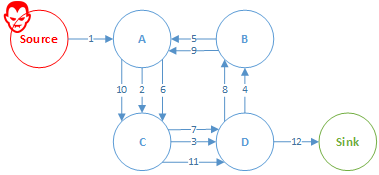
\includegraphics[width=0.8\linewidth]{figures/Carousel_Attack.png}
  \caption{Carousel Attack}
  \label{fig:carousel_attack}
\end{figure}

Existing mitigations strategies rely on checking the source route for loops on intermediary nodes, either selecting an appropriate route for the packet or simply dropping it.

\paragraph{\textbf{Stretch Attack}}
\paragraph{}
The objective of this attack is to create a longer source route around the network than the one who would be required to transverse the network from the source to the sink. The number of elements in the path would be greater than the optimal path, therefore increasing the total energy consumption by a factor of the number of additional hops. It's success rests on intermediary nodes not checking for better paths. Figure \ref{fig:stretch_attack} shows an example where a vampire node created a path that goes through a greater number of nodes than required to reach the sink.

\begin{figure}[h]
  \centering
  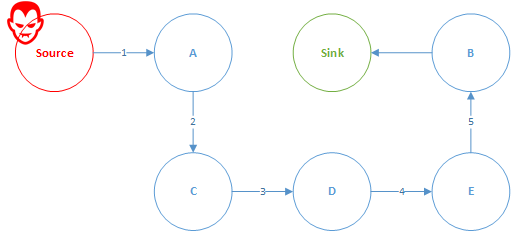
\includegraphics[width=0.8\linewidth]{figures/Stretch_Attack.png}
  \caption{Stretch Attack}
  \label{fig:stretch_attack}
\end{figure}

A limited way of mitigating this attack would be to ensure that path routes have less than the total number on devices on the network. Vasserman and Hoper proposed a property called "no-backtracking" that assures the packet is always moving closer to the sink on every hop. \cite{Vasserman2013}

\subsubsection{Stateful Protocols}
\paragraph{}
In systems that use this type of routing protocols, network nodes are aware of the network topology and it's state, being able to make local decisions on the node to whom they will forward the packet. The effect of the Vampires on this type of routing is limited since the route is built dynamically from many independent forwarding decisions. However, attackers can still cause damage by forcing packet forwarding through nodes that would not be on the optimal path, for example by forwarding the packet back to the source. A couple examples of these attacks are the Directional Antenna and Wormhole Attacks.

\paragraph{\textbf{Directional Antenna Attack}}
\paragraph{}
In this attack, the attacker takes the role of an intermediary and not the source of a packet. If the attacker has the resources to use a directional antenna, it can deposit a packet on arbitrary parts of the network while also forwarding the packet locally. This causes nodes that were not on the optimal path to also consume energy by forwarding a packet they would not normally receive, therefore increasing the total energy consumption by a factor of the directions the attacker can position the antenna and the distance between the receiver and the sink. Figure \ref{fig:directional_antenna_attack} shows an example where a vampire intermediary deposited a node on a distant location of the network, causing the packet to follow 2 different routes towards it's destination

\begin{figure}[h]
  \centering
  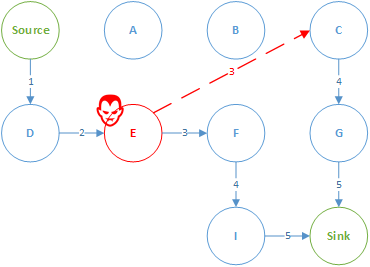
\includegraphics[width=0.8\linewidth]{figures/Directional_Antenna_Attack.png}
  \caption{Directional Antenna Attack}
  \label{fig:directional_antenna_attack}
\end{figure}

A mitigation strategy could be to analyse the route paths of a given packet that reached the sink more that one time. The last node identifier to appear duplicated before the path started to diverge would be one who then directed the packet to multiple regions, the attacker.

\paragraph{\textbf{Wormhole Attack}}
\paragraph{}

\subsubsection{RPL Specific Attacks}

\paragraph{\textbf{Hello Flooding}}

\paragraph{\textbf{Selective Forwarding}}

não sei onde meter, mas tem de aparecer aqui o clone attack...


\subsection{Secure Bootstrapping}
\paragraph{}
dizer o que é, de que forma se relaciona, que problemas resolve e um paragrafo com titulo a bold por cada forma que pode resolver o problema

